\chapter{Pruebas}
Las pruebas son una parte fundamental del desarrollo de software, ya que
permiten verificar el correcto funcionamiento del sistema y detectar posibles
errores antes de su implementación en un entorno de producción.

Con el objetivo de mejorar la calidad del sistema y tratar de encontrar posibles
defectos, se ha diseñado un plan de pruebas que permita verificar y
validar las diferentes funcionalidades del data lake. Este plan incluye pruebas
de despliegue, ingesta de datos, visualización y rendimiento, abarcando los
aspectos más críticos del sistema.

El plan de pruebas se ha diseñado siguiendo la técnica de clases de
equivalencia, que permite reducir el número de casos de prueba necesarios
mientras se mantiene una cobertura adecuada. Se han considerado diferentes
aspectos del sistema, desde el despliegue inicial hasta el rendimiento bajo
carga.


\newpage{}
\section{Plan de pruebas}
El plan de pruebas evalua diferentes aspectos del sistema, incluyendo el
despliegue, la ingesta de datos, la visualización y el rendimiento. Cada
aspecto se evalúa mediante pruebas de sistema y pruebas de carga, con el
objetivo de verificar el correcto funcionamiento del sistema en diferentes
condiciones.


El plan de pruebas se divide en dos categorías principales: pruebas de sistema
y pruebas de carga. Cada categoría incluye diferentes tipos de pruebas, con
objetivos específicos y casos de prueba asociados.

\begin{enumerate}
    \item \textbf{Pruebas de sistema:} verificar el correcto funcionamiento
        del sistema en diferentes escenarios. \begin{enumerate}
            \item Pruebas de despliegue
            \item Pruebas de visualización
            \item Análisis estático de código
        \end{enumerate}
    \item \textbf{Pruebas de carga:} evaluar el rendimiento del sistema bajo
        diferentes condiciones de carga. \begin{enumerate}
            \item Pruebas de ingesta de datos
            \item Pruebas de rendimiento
        \end{enumerate}
\end{enumerate}

A continuación, se detalla cada una de estas categorías, especificando los
objetivos, las clases de equivalencia consideradas y los casos de prueba
propuestos.


\newpage{}
\subsection{Pruebas de sistema}
Las pruebas de sistema evalúan el correcto funcionamiento del sistema en
diferentes escenarios, verificando que cumple con los requisitos y
especificaciones establecidas. Estas pruebas se centran en aspectos clave del
sistema, como el despliegue, la visualización y la calidad del código.

\subsubsection{Pruebas de despliegue}
Las pruebas de despliegue son cruciales para asegurar que el sistema puede ser
implementado correctamente en diferentes escenarios. Estas pruebas verifican
la robustez del proceso de despliegue y su capacidad para manejar diversas
condiciones iniciales.

\textbf{Objetivo:} Verificar que el sistema se despliega correctamente en
diferentes escenarios.

\paragraph{Clases de equivalencia}
\begin{itemize}
    \item Estado del sistema: Sin desplegar, en progreso de despliegue,
		desplegado
    \item Existencia de volúmenes: Sin volúmenes virtuales, con volúmenes
		virtuales montados
    \item Estado de puertos: Libres, Ocupados
    \item Cuenta en AWS: Sin cuenta configurada, con cuenta configurada
        incorrectamente, con cuenta configurada correctamente.
    \item Servicios disponibles: servicios no disponibles, Elasticsearch disponible,
        ES+Kibana disponible, Kafka disponible, todos disponibles\ldots
\end{itemize}

\paragraph{Casos de prueba}
\begin{enumerate}
    \item \textbf{DP-01:} Despliegue desde cero con todos los recursos libres
    \item \textbf{DP-02:} Intento de despliegue con sistema ya desplegado
    \item \textbf{DP-03:} Despliegue con volúmenes existentes y montados
    \item \textbf{DP-04:} Despliegue con puertos ocupados (\textcolor{red}{Inválido})
    \item \textbf{DP-05:} Despliegue sin cuenta de AWS configurada (\textcolor{red}{Inválido})
    \item \textbf{DP-06:} Despliegue con cuenta de AWS mal configurada (\textcolor{red}{Inválido})
\end{enumerate}


\newpage{}
\subsubsection{Pruebas de visualización}
La visualización efectiva de los datos es esencial para que los usuarios
puedan obtener insights valiosos. Estas pruebas evalúan la capacidad básica
de Kibana para visualizar los datos ingestados.

Las pruebas de visualización son, conceptualmente, pruebas \textit{end-to-end},
ya que verifican que los datos ingestados se visualizan correctamente en la
herramienta de visualización.

\textbf{Objetivo:} Verificar que los datos ingestados se visualizan
correctamente en Kibana.

\paragraph{Clases de equivalencia}
\begin{itemize}
    \item Tipo de visualización: Gráficos de barras, gráficos de líneas,
        tablas, paneles de control
    \item Complejidad de la consulta: Simple, ``compleja''
    \item Volumen de datos visualizados: Pequeño, ``grande''
\end{itemize}

\paragraph{Casos de prueba}
\begin{enumerate}
    \item \textbf{VIS-01:} Creación de un gráfico de barras simple con pocos datos
    \item \textbf{VIS-02:} Generación de un panel de control complejo con datos de múltiples fuentes
    \item \textbf{VIS-03:} Visualización de una tabla con gran volumen de datos
\end{enumerate}


\newpage{}
\subsubsection{Análisis estático de código}
El análisis estático de código es una técnica que permite detectar posibles
errores y problemas en el código fuente sin necesidad de ejecutarlo. Estas
pruebas evalúan la calidad del código y su cumplimiento de las normas de
programación.

En el caso de este proyecto, se analiza de manera constante el código fuente
mediante SonarQube, una herramienta de análisis estático de código que permite
identificar problemas de calidad y seguridad en el código.

\begin{figure}[H]
	\centering
	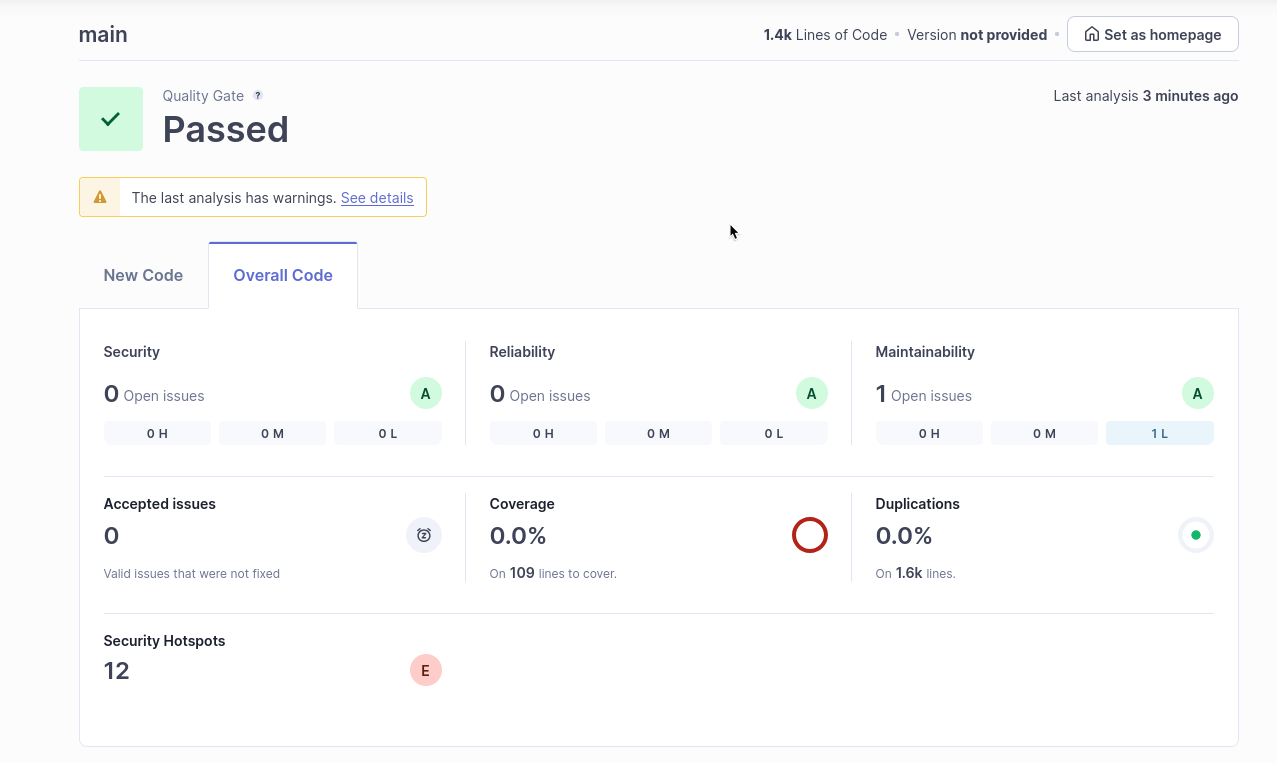
\includegraphics[width=\textwidth]{pruebas/sonar_gate.png}
	\caption{Análisis estático de código con SonarQube}
	\label{fig:sonarqube}
\end{figure}

SonarQube analiza la calidad de cada versión en base a un conjunto de reglas
predefinidas (\textit{quality gate}), y muestra un informe detallado con los
problemas encontrados y sugerencias para su corrección.

Se utiliza la máquina especializada de SonarQube de la empresa, desplegada y
mantenida por el alumno, para analizar el código de manera automatizada mediante
las \textit{pipelines} de Bitbucket cada vez que se publica un cambio al
repositorio.


\newpage{}
\subsection{Pruebas de carga}
\subsubsection{Pruebas de ingesta de datos}
La ingesta de datos es una funcionalidad central del data lake. Estas pruebas
están diseñadas para verificar la capacidad del sistema para procesar datos de
diferentes fuentes, volúmenes y frecuencias.

\textbf{Objetivo:} Comprobar que el sistema ingesta correctamente datos de
diferentes fuentes.

\paragraph{Clases de equivalencia}
\begin{itemize}
    \item Tipo de fuente: MySQL, MongoDB, Logs de Laravel, Logs de AWS ELB
    \item Volumen de datos: Pequeño ($<1000$ registros), Mediano ($1000-100000$
    	registros), Grande ($>100000$ registros)
    \item Frecuencia de ingesta: Baja (cada hora), Media (cada minuto), Alta
    	(tiempo real)
\end{itemize}

\paragraph{Casos de prueba}
\begin{enumerate}
    \item \textbf{IN-01:} Ingesta de pequeño volumen de logs de MySQL
    \item \textbf{IN-02:} Ingesta de gran volumen de datos de MongoDB
    \item \textbf{IN-03:} Ingesta en tiempo real de logs de Laravel
    \item \textbf{IN-04:} Ingesta periódica de logs de AWS ELB
\end{enumerate}


\newpage{}
\subsubsection{Pruebas de rendimiento}
El rendimiento del sistema es crítico, especialmente cuando se manejan grandes
volúmenes de datos o múltiples consultas simultáneas. Estas pruebas evalúan
cómo responde el sistema bajo diferentes condiciones de carga.

Para realizar estas pruebas de carga, se manipulan los scripts de ingesta de
carga (ver \fullref{anexo:kafka}) y se utiliza la herramienta de estrés de
carga \textit{Locust}, otra herramienta desplegada y mantenida por el alumno
dentro de la nube de servicios de la empresa. Al crear picos de carga en el
\textit{backend}, se aumenta la cantidad de registros en \textit{AWS CloudWatch},
que a su vez se ingestan a través del sistema establecido.

También se prueba la capacidad de respuesta del sistema mediante la ejecución
de múltiples consultas simultáneas en Kibana mediante múltiples navegadores y
usuarios.

\textbf{Objetivo:} Evaluar el rendimiento del sistema bajo diferentes cargas.

\paragraph{Clases de equivalencia}

\begin{itemize}
    \item Carga de ingesta: Baja ($<100$ eventos/min), media ($100-1000$ eventos/min),
    	alta ($>=1000$ eventos/min)
    \item Carga de consultas: Pocas consultas simultáneas ($<10$), Muchas
    consultas simultáneas ($>=10$)
\end{itemize}

\paragraph{Casos de prueba}
\begin{enumerate}
    \item \textbf{PERF-01:} Ingesta de alta carga de eventos durante 1 hora
    \item \textbf{PERF-02:} Ejecución de múltiples consultas complejas simultáneas
    \item \textbf{PERF-03:} Combinación de alta carga de ingesta y consultas simultáneas
\end{enumerate}


\newpage{}
\section{Ejecución de pruebas}
La ejecución de las pruebas se lleva a cabo de manera sistemática, siguiendo
el plan establecido. Para cada caso de prueba, se documentaron los siguientes
aspectos:

\begin{enumerate}
    \item Pasos de ejecución
    \item Resultado esperado
    \item Resultado obtenido
    \item Estado (Pasado/Fallido)
\end{enumerate}

A continuación, se presenta un ejemplo de ejecución de una prueba, incluyendo
los pasos y resultados esperados y obtenidos, y posteriormente se presenta una
tabla resumen con los resultados de todas las pruebas realizadas.


\newpage{}
\subsection{Ejemplo de ejecución}
\textbf{Despliegue desde cero con todos los recursos libres (DP-01)}
Esta prueba es la más básica de las pruebas de despliegue, y tiene como
objetivo verificar que el sistema se puede desplegar correctamente en un
entorno limpio, sin recursos previamente desplegados.

\subsubsection{Pasos de ejecución}
\begin{itemize}
    \item Asegurar que no hay recursos desplegados previamente
    \item Configurar correctamente las credenciales de AWS
    \item Ejecutar el comando \texttt{terraform init}
    \item Ejecutar el comando \texttt{terraform apply}
\end{itemize}

\subsubsection{Resultado esperado}
\begin{itemize}
    \item Terraform debe completar el despliegue sin errores
    \item Todos los recursos (ECS, Elasticsearch, Kibana, Logstash, Kafka)
    deben estar en estado "running"
    \item Se deben poder acceder a las interfaces web de Kibana y Elasticsearch
\end{itemize}

\subsubsection{Resultado obtenido}
\begin{itemize}
    \item Terraform completó el despliegue sin errores
    \item Todos los recursos se desplegaron correctamente y están en estado
    "running"
    \item Se pudo acceder a Kibana y Elasticsearch a través de sus respectivas
    URLs
\end{itemize}

\subsubsection{Estado} \textcolor{green}{Pasado}

Este resultado exitoso indica que el proceso de despliegue automatizado
funciona correctamente y es capaz de configurar todos los componentes
necesarios del sistema de manera eficiente.


\newpage{}
\subsection{Tabla de resultados}
A continuación, se presenta una tabla resumen con los resultados de la
ejecución de todas las pruebas planificadas, incluyendo las pruebas de
despliegue, ingesta de datos, visualización y rendimiento.

\begin{table}[h]
    \centering
    \begin{tabular}{|p{1.5cm}|p{5cm}|p{5cm}|p{2cm}|}
        \hline
        \textbf{ID} & \textbf{Prueba} & \textbf{Resultado} & \textbf{Estado} \\
        \hline
        DP-01 & Despliegue desde cero &
        Recursos desplegados y accesibles &
        \cellcolor{green!25}OK \\
        \hline
        DP-02 & Redespliegue con sistema existente &
        Sin cambios realizados &
        \cellcolor{green!25}OK \\
        \hline
        DP-03 & Despliegue con volúmenes existentes &
        Volúmenes reutilizados &
        \cellcolor{green!25}OK \\
        \hline
        DP-04 & Despliegue con puertos ocupados &
        Error de puertos mostrado &
        \cellcolor{green!25}Error (OK) \\
        \hline
        DP-05 & Despliegue sin cuenta AWS &
        Error de credenciales &
        \cellcolor{green!25}Error (OK) \\
        \hline
        DP-06 & Despliegue con cuenta AWS incorrecta &
        Error de credenciales &
        \cellcolor{green!25}Error (OK) \\
        \hline
        IN-01 & Ingesta logs MySQL &
        Logs en Elasticsearch &
        \cellcolor{green!25}OK \\
        \hline
        IN-02 & Ingesta masiva MongoDB &
        Datos ingestados sin pérdidas &
        \cellcolor{green!25}OK \\
        \hline
        IN-03 & Ingesta tiempo real Laravel &
        Logs visibles, retraso $<5$s &
        \cellcolor{green!25}OK \\
        \hline
        IN-04 & Ingesta periódica AWS ELB &
        Logs cada 5min &
        \cellcolor{green!25}OK \\
        \hline
        \hline
        VIS-01 & Gráfico de barras simple &
        Gráfico creado correctamente &
        \cellcolor{green!25}OK \\
        \hline
        VIS-02 & Panel control complejo &
        Panel con 4 fuentes de datos &
        \cellcolor{green!25}OK \\
        \hline
        VIS-03 & Tabla gran volumen &
        1M registros en $<3$s &
        \cellcolor{green!25}OK \\
        \hline
        \hline
        PERF-01 & Ingesta alta carga 1h &
        1M eventos/min sin pérdidas &
        \cellcolor{green!25}OK \\
        \hline
        PERF-02 & Consultas complejas simultáneas &
        20 consultas, respuesta $<2$s &
        \cellcolor{green!25}OK \\
        \hline
        PERF-03 & Carga mixta &
        500k/min + 10 consultas, $<3$s &
        \cellcolor{green!25}OK \\
        \hline
    \end{tabular}
    \caption{Ejecución de pruebas del sistema}
    \label{tab:pruebas}
\end{table}

La ejecución completa de las pruebas se realiza una vez completada la
implementación del sistema, pero son pruebas similares a las que se han
realizado durante el desarrollo del mismo, con el objetivo de asegurar que el
sistema cumple con los requisitos y especificaciones establecidas.
